\documentclass[11pt]{beamer}
\usetheme{Goettingen}
\usepackage[utf8]{inputenc}
\usepackage{amsmath}
\usepackage{amsfonts}
\usepackage{amssymb}
\usepackage{graphicx}
\usepackage{hyperref}
\usepackage{extarrows}
\usepackage[hang,flushmargin]{footmisc}

\title{Point Group Equivariant Convolutional Graph Neural Networks}
\author{Alex Heilman}
%\setbeamercovered{transparent} 
%\setbeamertemplate{navigation symbols}{} 
%\logo{} 
%\date{} 
\addtobeamertemplate{navigation symbols}{}{%
    \usebeamerfont{footline}%
    \usebeamercolor[fg]{footline}%
    \hspace{1em}%
    \insertframenumber/\inserttotalframenumber
}


\usepackage[style=numeric,backend=bibtex]{biblatex}
\addbibresource{chgcnn.bib}

\newenvironment{boxed2}
    {\begin{center}
    \begin{tabular}{|p{0.95\textwidth}|}
    \hline\\
    }
    { 
    \\\\\hline
    \end{tabular} 
    \end{center}
    }


\renewbibmacro*{\tiny cite:title}{\tiny%
  \printtext[bibhyperref]{%
    \printfield[citetitle]{labeltitle}%
    \setunit{\space}%
    \printtext[parens]{\printdate}%
  }%
}

\begin{document}

\begin{frame}
\titlepage
\end{frame}

%\begin{frame}
%\tableofcontents
%\end{frame}

\begin{frame}{Overview}
\begin{itemize}
	\item Brief review of mathematics
	\item Group representation theory
	\begin{itemize}
	\item Irreps
	\item Basis Functions
	\item Coupling Coefficients
	\end{itemize}
	\item Equivariant networks
	\begin{itemize}
		\item $SO(3)$ Equivariance
	\end{itemize}
	\item Applications

\end{itemize}
\end{frame}

\section{Groups and Vector Spaces}

\begin{frame}{Group Definition}
	A group $G$ is a set of elements $\lbrace g_1, ..., g_n\rbrace$ with a binary operation $*:G\times G \rightarrow G$ between elements that satisfies the conditions of identity, associativity, invertability, and closure.
	
	\begin{boxed2}
		
		\vspace{-.5cm}
		
		\textbf{Example: General Linear Group}
		
		The general linear group $GL(V)$ formed over some vector space $V$ is the set of non-singular $d_v\times d_v$ matrices acting on $V$ with the group operation being matrix multiplication. The general linear group is itself a vector space.
	\end{boxed2}
\end{frame}

\begin{frame}{Vector Space Definition}
	A vector space $V$ over a field $K$ is a group of vectors equipped with a distributive scalar multiplication. Vectors are often defined by way of a basis set that spans the space under scalar multiplication.
	

	\begin{boxed2}
		
		\vspace{-.61cm}
		
		\textbf{Example: $\mathbb{R}^3$, Real 3 Dimensional Space} 
		
		Locations in physical space may be modeled with a three dimensional vector space  $\mathbb{R}^3$ over the real numbers $\mathbb{R}$ with basis functions $\hat{x},\hat{y},\hat{z}$.
		
		\vspace{-.3cm}
		
	\end{boxed2}	
	
	
		\begin{boxed2}
		
		\vspace{-.61cm}
		
		\textbf{Example: Functions on Real 3 Dimensional Space} 
		
		Scalar functions on physical space also form a vector space over the real numbers, albeit infinite-dimensional. In this case, the group operation between vectors (functions) is point-wise addition.
		
		\vspace{-.3cm}
		
	\end{boxed2}	
	
We may construct new vector spaces from sets of existing vector spaces by taking tensor products and direct sums.

\end{frame}



%\begin{frame}{Cartesian Products}
%	content...
%\end{frame}

\begin{frame}{Direct Sums}
We may form direct sums $V\oplus W$ of vector spaces $V,W$ by block-diagonal concatenation. This operation enjoys scalar distributivity to respective subspaces with the set of scalars $K_V\oplus K_W$.

\begin{boxed2}
	
	\vspace{-.57cm}
	
	\textbf{Example: Direct Sum of Matrices}
	
	
	\vspace{-.12cm}
	
	$$
		\begin{bmatrix}
			a_1&b\\
			c&a_2\\
		\end{bmatrix}
		\oplus 
		\begin{bmatrix}
			d_1&0\\
			0&d_2\\
		\end{bmatrix}
		=\begin{bmatrix}
			a_1&b&0&0\\
			c&a_2&0&0\\
			0&0 &d_1 &0\\
			0&0&0&d_2\\
		\end{bmatrix}
	$$

\vspace{-.1cm}

\end{boxed2}
	
Direct sums of vector spaces are themselves vector spaces.
\end{frame}

\begin{frame}{Tensor Products}
Tensor products $V\otimes W$ of vector spaces $V,W$ are uniquely bilinear so that $\lambda V\otimes W = V\otimes\lambda W = \lambda (V\otimes W)$. 
\begin{boxed2}
	
	\vspace{-.57cm}
	
	\textbf{Example: Tensor Product of Matrices}
	
	Also known as "Kronecker Product".
	
	
	\vspace{-.12cm}
	
	$$
	\begin{bmatrix}
		a_1&b\\
		c&a_2\\
	\end{bmatrix}
	\otimes 
	\begin{bmatrix}
		d_1&0\\
		0&d_2\\
	\end{bmatrix}
	=\begin{bmatrix}
		a_1d_1&0&bd_1&0\\
		0&a_1d_2&0&bd_2\\
		cd_1&0 &a_2d_1 &0\\
		0&cd_2&0&a_2d_2\\
	\end{bmatrix}
	$$
	
	\vspace{-.3cm}
	
\end{boxed2}

Tensor products of vector spaces are themselves vector spaces.
\end{frame}


\section{Representation Theory}
\begin{frame}{Group Representations}
	A representation $\rho_G$ of a group $G$ is a homomorphism from elements $g$ to a set of linear operators (square matrices). 
	
	\vspace{0.25cm}\small
	
		\begin{boxed2}
		
		\vspace{-.5cm}
		
		\textbf{Example: 3D Representation of $C_3$}
		
		Consider three identical points in 3D space forming an equilateral triangle.
		\begin{center}
			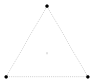
\includegraphics[scale=0.2]{c3triangle.pdf}
		\end{center}
		These clearly are symmetrical under three-fold rotations about the origin in the xy plane. These $C_3$ group actions act on this Cartesian basis with the representation $\rho$ defined:\tiny
		
		$$
		\rho(\mathbb{I}) = \begin{bmatrix}
			1&0&0\\
			0&1&0\\
			0&0&1\\
		\end{bmatrix}\quad 		\rho(C_3) = \begin{bmatrix}
		-\frac{1}{2}&-\frac{\sqrt{3}}{2}&0\\
		\frac{\sqrt{3}}{2}&-\frac{1}{2}&0\\
		0&0&1\\
		\end{bmatrix}\quad 
		\rho(C_3^2) = \begin{bmatrix}
		-\frac{1}{2}&\frac{\sqrt{3}}{2}&0\\
		-\frac{\sqrt{3}}{2}&-\frac{1}{2}&0\\
		0&0&1\\
		\end{bmatrix}
		$$
		
		\vspace{-0.5cm}
		
	\end{boxed2}
\end{frame}


\begin{frame}{Irreducible Representations (IRs)}
	For atomic arrangements, 3D group representations $\rho$ are  often reducible in terms of a direct sum of 'smaller' group representations $\rho^{(\alpha)}$:
	$$
	\rho = \bigoplus_{\alpha}c_{\alpha}\rho^{(\alpha)}
	$$
	
	Maschke's theorem guarantees that any given representation is always decomposable as a direct sum of irreducible representations. 

	\vspace{0.3cm}
	
	This set may always be taken to satisfy:
	
	\medskip
	
	$\bullet$ Unitarity
	
	\medskip
	
	$\bullet$ Orthogonality
	
	\medskip
	
	$\bullet$ $\sum_{\alpha} d_{\alpha}^2 = N $ where $d_{\alpha} $ is the dimension of IR $\alpha$ and $N$ is the order
	
\end{frame}

\begin{frame}{IRs (cont.)}

\begin{boxed2}
	
	\vspace{-.57cm}
	
	\textbf{Example: IRs of $D_3$} The previously shown representation of $C_3$ elements is reducible into a two-dimensional subspace and a one-dimensional subspace of $D_3$. 
	
	\vspace{-.12cm}

$$
\rho(\mathbb{I}) =
\rho^{(2)}(\mathbb{I})\oplus\rho^{(1)}(\mathbb{I})
=
\begin{bmatrix}
1&0\\
0&1\\
\end{bmatrix}
\oplus 
\begin{bmatrix}
1
\end{bmatrix}
$$
$$
\rho(C_3)
=\rho^{(2)}(C_3)\oplus\rho^{(1)}(C_3)=
\begin{bmatrix}
	-\frac{1}{2}&-\frac{\sqrt{3}}{2}\\
	\frac{\sqrt{3}}{2}&-\frac{1}{2}\\
\end{bmatrix}
\oplus
\begin{bmatrix}
	1
\end{bmatrix}
$$
$$
\rho(C_3^2) 
=
\rho^{(2)}(C_3^2)\oplus\rho^{(1)}(C_3^2)
= 
\begin{bmatrix}
	-\frac{1}{2}&\frac{\sqrt{3}}{2}\\
	-\frac{\sqrt{3}}{2}&-\frac{1}{2}\\
\end{bmatrix}
\oplus
\begin{bmatrix}
	1
\end{bmatrix}
$$
	
	\vspace{-.3cm}
	
\end{boxed2}
\end{frame}

\begin{frame}{Equivalence Classes}
Equivalence classes are subsets of group elements that mutually exchange under conjugation, where element $g$ conjugated by element $h$ means:
$$
g\rightarrow hgh^{-1}
$$
In the space of a representation, this is referred to as a similarity transformation, which is essentially a change of basis.

\medskip

Note that the number of equivalence classes $N_c$ is equal to the number of irreducible representations.
$$
N_{\text{IR}} = N_{c}
$$
\end{frame}

\begin{frame}{Character Tables}
	Irreducible representations are only unique up to change of basis, but their traces are invariant.
	
	$$
	\chi^{(\alpha)}(g)= \text{Tr}\big(\rho^{(\alpha)}(g)\big)
	$$
	
	The trace of a representation is known as it's character $\chi$, which is unique for equivalence classes $\langle g \rangle$.
	
	
		\begin{boxed2}
		
		\vspace{-.57cm}
		
		\textbf{Example: $C_4$ Character Table}
		
		\vspace{-.12cm}
		
		$$
		\begin{array}{c|c c c c}
			C_4 & \langle \mathbb{I}\rangle  & \langle C_4\rangle  & \langle C_4^2\rangle  & \langle C_4^3\rangle \\
			\hline 
			a_1 & 1 & 1 & 1 & 1 \\
			a_2 & 1 & -1 & 1 & -1 \\
			a_3 & 1 & i & -1 & -i \\
			a_4 & 1 & -i & -1 & i \\
		\end{array}
		$$
		
		\vspace{-.3cm}
		
	\end{boxed2}
		
	Characters are often displayed in 'character tables', with IRs on one axis and equivalence classes along the other.
	
\end{frame}

\begin{frame}{Orthogonality Theorems}
	IRs are orthogonal in the following ways:
	$$
	\frac{1}{N}\sum_{g}\chi^{(\alpha)*}(g)\chi^{(\beta)}(g) = \delta_{\alpha\beta}
	$$
	$$
	\sum_{\alpha}\chi^{(\alpha)*}(c_k)\chi^{(\alpha)}(c_h)= \frac{N}{N_k}\delta_{kh}
	$$
	where $N$ is the number of elements in $G$ and $N_k$ is the number of elements in equivalence class $k$.
	
	\medskip
	
	This allows us to decompose reducible representations by determining the coeffecients of expansion $c_{\alpha}$ as:
	
	$$
	c_{\alpha} = \frac{1}{N}\sum_{g}\chi^{(\alpha)*}(g)\chi(g)
	$$ 
\end{frame}

\begin{frame}{Orthogonality Theorems (cont.) }
	\small
\begin{boxed2}
	
	\vspace{-.41cm}
	
	\textbf{Example: d-shell Splitting in Octohedral Coordinations} 
	
	Take the Hydrogen-like orbitals $\psi_{\ell m}$ as a basis for spherically symmetric states. The d-shell orbitals are the basis functions of the $\ell=2$ representations.
	
	\medskip
	
%conventionally given as:
%	$$
%	\lbrace xy, xz, yz, 2z^2-x^2-y^2, x^2-y^2 \rbrace
%	$$
	The octohedral complex's symmetry group is $O$, with it's character table and the $\Gamma^{\ell=2}$ representation:
	$$
	\begin{array}{c|c c c c c}
		O & 1\langle \mathbb{I}\rangle  & 8\langle C_3\rangle  & 3\langle C_2\rangle  & 6\langle C_2'\rangle & 6\langle C_4^3\rangle \\
		\hline 
		(d)\ \Gamma^{\ell=2} & 5 & -1 & 1 & 1 & -1 \\
		A_1 & 1 &  1&  1&  1&  1\\
		A_2 & 1&  1&  1&  -1&  -1\\
		E & 2 & -1 & 2 & 0 & 0 \\
		T_1 & 3 & 0 & -1 & -1 &1\\
		T_2 & 3 & 0 & -1 & 1 &-1\\
	\end{array}
	$$
	Orthogonality then gives $\gamma^{\ell=2}=E\oplus T_2$. In practice, this results in a 5-fold degeneracy being lifted into a two- and three-fold degeneracy.
	
	\vspace{-.3cm}
	
\end{boxed2}
\end{frame}
\begin{frame}{Basis Functions}
	Every representation of a group inherits a vector space on which it has a natural action. This vector space is spanned by a chosen set of basis functions $\vert \psi^{\alpha}_i\rangle$.

	\vspace{0.5cm}
	
	\begin{itemize}
		\item 	An irrep $\Gamma^{\alpha}$'s components are determined by basis:
		$$\Big(\Gamma^{\alpha}(g)\Big)_{i}^{j}=\langle\psi^{\alpha}_j\vert \Gamma^{\alpha}(g) \vert \psi^{\alpha}_i\rangle$$
		
		\item Basis functions are said to ``transform as an irrep $\alpha$" if:
		$$
		\Gamma^{\alpha}(g) \vert \psi^{\alpha}_i\rangle =\sum_{j} \Big(\Gamma^{\alpha}(g)\Big)^j_i \vert \psi^{\alpha}_j\rangle
		$$
	\end{itemize}
	

\end{frame}


\begin{frame}{Basis Functions (cont.)}
		\small

	\begin{boxed2}
		
		\vspace{-.5cm}
		
		\textbf{Example: $3D$ Basis Functions of $D_3$}
		
		Consider previous $3D$ representation of $C_3$ rotations in $D_3$, which act on vectors $\vec{r}_{\rho}$:
		$$
		\vec{r}_{\rho}=\begin{bmatrix}
			x\\y\\z
		\end{bmatrix} = \vec{r}_{\rho^{(2)}}\oplus\vec{r}_{\rho^{(1)}} =\begin{bmatrix}
		x\\y
		\end{bmatrix}\oplus\begin{bmatrix}
		z
		\end{bmatrix}
		$$
		Clearly, $x,y$ is a basis transforming as $\Gamma^{2}$ and $z$ is a basis for $\Gamma^1$.

	\end{boxed2}
	
		\begin{boxed2}
		
		\vspace{-.41cm}
		
		\textbf{Example: Tight Binding} 
		
		The tight binding approximation often uses localized Hydrogen-like orbitals $\psi_{nm}^{\ell}$ as a basis for many-body systems
		
		\vspace{-.3cm}
		
	\end{boxed2}
	
\end{frame}

\begin{frame}{Projection Operators}
	If we have an explicit form for IR $\alpha$, we may project an arbitrary function onto the $k$-th basis function $f^{\alpha}_k$ of IR $\alpha$ with $\hat{P}_{\alpha}^{kk}$:
	$$
	\hat{P}_{\alpha}^{kk} = \frac{d_{\alpha}}{N}\sum_g \big[\Gamma^{kk}_{\alpha}(g) \big]^* O(g)
	$$
	where $d_{\alpha}$ is the dimensional of IR $\alpha$, and then we have:
	$$
	f_{\alpha}^k(\vec{r}) = \hat{P}_{\alpha}^{kk}f(\vec{r})
	$$
	From the characters alone, we may project a function onto it's total $\alpha$ subspace with $\hat{P}_{\alpha}$:
	$$
	\hat{P}_{\alpha} = \sum_k\hat{P}^{kk}_{\alpha} = \frac{d_{\alpha}}{N}\sum_{g}\chi^{(\alpha)*}(g)\hat{O}(g)
	$$


\end{frame}

\begin{frame}{Coupling Coefficients}
Consider a direct product decomposition of some irreps $\Gamma$:
$$
\Gamma^{\alpha}\otimes\Gamma^{\beta}=\bigoplus_{\gamma}c_{\alpha\beta\gamma}\Gamma^{\gamma}
$$
	
Products of basis functions $u^{\alpha}_iv^{\beta}_j$ then decompose similarly into a direct sum of irreps with basis functions $\psi_{n}^{\gamma}$ via the coupling coefficients $U_{\alpha i \beta j}^{\gamma n}$ as:
$$
\psi_{n}^{\gamma}= \sum_{i,j}U_{\alpha i \beta j}^{\gamma n}u^{\alpha}_iv^{\beta}_j
$$

	\begin{boxed2}\tiny
	
	\vspace{-.61cm}
	
	\textbf{Example: Clebsch-Gordan Coefficients} 
	
	The Clebsch-Gordan coefficients $C^{\ell_f  m_f}_{\ell_1  m_1\ell_2 m_2}$ are the coupling coefficients of $SO(3)$, which relate tensor product spaces of spherical harmonics $Y^{\ell}_m$ to direct sums of spherical harmonics.
	$$
	Y_{\ell_1}^{m_1}(\Omega)Y_{\ell_2}^{m_2}(\Omega)=\sum_{\ell_3, m_3}\sqrt{\frac{(2\ell_1+1)(2\ell_2+1)}{4\pi(2\ell_3+1)}}C^{\ell_3m_3}_{\ell_1m_1\ell_2m_2}C^{\ell_30}_{\ell_1 0\ell_2 0}Y_{\ell_3m_3}(\Omega)
	$$
	
	\vspace{-.3cm}
	
\end{boxed2}

\end{frame}

\begin{frame}{Coupling Coefficients (cont.)}
	Dirl's Formula \cite{dirl1979}:\footnotesize
	$$
	(U^{\gamma n}_{\alpha i \beta j})^m = \sqrt{\frac{d_{\gamma}}{N_{G}}}\Big[\sum_{g\in G}\Gamma^{\alpha}_{qq}(g)\Gamma^{\beta}_{ss}(g)\Gamma^{\gamma \dagger}_{aa}(g)\Big]^{-\frac{1}{2}}\cdot \sum_{g\in G}\Gamma^{\alpha}_{iq}(g)\Gamma^{\beta}_{js}(g)\Gamma^{\gamma\dagger}_{na}(g)
	$$
\end{frame}

\section{Group Equivariant Networks}
\begin{frame}{Equivariant Functions}
	An equivariant function $f:X\rightarrow Y$, where $X,Y$ are vector spaces, is one that 'commutes' with a group's actions, satisfying:
	$$
	f\Big(\mathcal{D}^X(g)x\Big)=\mathcal{D}^Y(g)f(x)
	$$
	Tensor products are uniquely equivariant with respect to their argument vector spaces.
\end{frame}
\begin{frame}{Why Equivariant Functions?}
	Physics assumes there exists a map between configurations and properties of physical systems: 
	$$
	  \lbrace\vec{r}_i \rbrace \xrightarrow[\text{Nature}]{}
	  \lbrace\vec{r}_i' \rbrace
	$$
	Neural network techniques assume maps between abstract input and output spaces exist:
	$$
	X
	\xrightarrow[\text{Neural Network}]{}
	Y
	$$
	and that these may be expressed in a basis of adequately large neural networks.
\end{frame}
\begin{frame}{Why Equivariant Functions? (cont.)}
	\begin{center}
	Physical processes respect coordinate system rotations $R$:
	$$
	\lbrace R\vec{r}_i \rbrace \xrightarrow[\text{Nature}]{}
	\lbrace R\vec{r}_i' \rbrace
	$$
	In general, neural networks do not:
	$$
	RX
	\xrightarrow[\text{Neural Network}]{} \ \ 
	?
	$$
	
	So what do we want?

	\end{center}
\end{frame}
\begin{frame}{Equivariant Networks}
\begin{center}
We want equivariant networks for physics!

	$$
	RX
	\xrightarrow[\text{Neural Network}]{\text{Equivariant}} RY
	$$
	
\vspace{0.6cm}

\end{center}
	
In equivariant networks, we consider feature vectors in basis of representation space as:
$$
v^{\alpha}_i
$$
with indexes $\alpha$ denoting the irrep it transforms as, and $i$ denoting the dimension of irrep space $\alpha$.
\end{frame}
\begin{frame}{Equivariant Networks (cont.)}
Compositions of equivariant functions are equivariant \cite{tacovariant}. We consider building blocks:{\small
\begin{itemize}

	\item Self-interaction:
	$$
	v'_{nc} = W^i_c v_{ni}
	$$
	\item Non-linear functions along channels  (for trivial irrep $\alpha=1$):
	$$
	v'_{nc}=f(v_{nc}+b_{nc})
	$$
	\item Group correlation with filters:
	$$
	[F\star v](g)=\sum_{h\in G}\sum_c F_c(h)v_c(g^{-1}h)
	$$
	\item Tensor products with filters:
	$$
	(v'_{nc})^{\gamma}_{n} = \sum_{ij}U_{\alpha i \beta j}^{\gamma n}\big(F_{j}^{\beta}\otimes V^{\alpha}_i \big) 
	$$
	\item Pooling over nodes or channels:
	$$
	v_c = \sum_n v_{nc}
	$$
\end{itemize}}
\end{frame}
\begin{frame}{$SO(3)$ Properties}
Most modern equivariant networks are specifically $SO(3)$-Equivariant.

\vspace{0.5cm}

\begin{itemize}
\item Inifinite order $\rightarrow$ infinite irreps
\item Irreps are Wigner $\mathcal{D}^{\ell}$ matrices
\item Natural basis set $Y^{\ell}_m$ of dimension $d_{\ell}=2\ell+1$
\end{itemize}

\vspace{0.5cm}

Many models are further referred to as $E(3)$-equivariant for the Euclidean group (add parity and translation invariance).
\end{frame}

\begin{frame}{\textit{Tensor Field Networks}}
	Tensor field networks \cite{tfn} use SO(3) equivariant convolution:{\small
	$$
	\big(v^{L+1}_{nc}\big) ^{\ell}_{m}=\big(v^{L}_{nc}\big)^{\ell}_m+\sum_{b\in \mathcal{N}(n)}\sum_{\ell_f m_f , \ell_i m_i}^{\ell_{\text{max}} m_{\text{max}}}c_{\ell_fm_f\ell_im_i}^{\ell m}\big(F^{L}_c(r_{nb})\big)^{\ell_f}_{m_f}\big(v_{bc}^L \big)^{\ell_i}_{m_i}
	$$}
	\begin{itemize}
		\item $v_{nc}^{L}$: Node feature of node $n$, channel $c$, layer $L$
		\item $c_{\ell_fm_f\ell_im_i}^{\ell_om_o}$: Clebsch-Gordan coefficients
		\item $F_c^L$: Filter function (trainable)
		\item $r_{nb}$: Radius between nodes $n$ and neighbor $b\in \mathcal{N}(n)$
	\end{itemize}
	
	\vspace{.7cm}
	
	$F$ is generally a neural network; $r$ is often expanded with some radial basis function (RBF): Gaussian, Bessel, etc.
\end{frame}

\section{Point Groups and Space Groups}

\begin{frame}{Point Group Properties}
Groups of operations that leave at least one point fixed and are compatible with a Bravais lattice.

\vspace{0.3cm}
	
Point groups (in 3D) have following properties:
	\begin{itemize}
		\item 32 crystallographic point groups in 3D
		\item Finite number of irreps for each
		\item All irreps of point groups are of dimension $d_{\alpha}=1,2,3$
		\item All allow a (often reducible) 3D representation
		\item Decompositions with $c_{\alpha\beta\gamma}=0,1,2$
	\end{itemize}
	
{\small
(Point group representations may be used to generate induced representations of space groups)}
\end{frame}

\begin{frame}{Site-symmetry Equivariant Networks}
\begin{center}
	Index vectors by $\alpha ,i$  from site-symmetry group instead!
\end{center}
{\small
	$$
	\big(v^{L+1}_{nc}\big) ^{\ell}_{m}=\big(v^{L}_{nc}\big)^{\gamma}_n+\sum_{b\in \mathcal{N}(n)}\sum_{\alpha i, \beta j}U_{\alpha i \beta j}^{\gamma n}\big(F^{L}_c(r_{nb})\big)^{\beta }_{j}\big(v_{bc}^L \big)^{\alpha}_{i}
	$$}
	
\begin{itemize}
	\item Natural cutoff (finite summation over $\alpha,\beta$)
	\item Natural readout for symmetric properties ($\gamma=1$)
	\item Accounts for all physical symmetry but not more
\end{itemize}

\end{frame}


\begin{frame}{Space Groups}
Semidirect product of point group $R$ and lattice translation group $T$:
$$
G = T\ltimes R
$$
\begin{itemize}
	\item Describes all symmetries of crystals
	\item Infinite order $\rightarrow$ infinite irreps
	\item Can learn features associated with point group and induce for space group
\end{itemize}

\end{frame}

\begin{frame}{Induced Representations}
	\begin{center}
	"Opposite of a reduced representation"
	\end{center}

\vspace{0.15cm}

Use subgroup $G$ representation $\tilde{\rho}$ to form representation $\rho$ of parent $H$:
$$
\rho_{\alpha i ,\beta j}(h) = \begin{cases}
\ \ \tilde{\rho}(g)_{ij}	\quad\text{if } h_{\alpha}^{-1}h h_{\beta}=g\in G \\ 
\ \ 0 \quad \quad \quad  \text{else} \\
\end{cases}
$$
where $\alpha$ indexes a coset decomposition of $H$  into $G\subset H$.


\begin{boxed2}
	
	\vspace{-.61cm}
	\footnotesize
	\textbf{Example: Induced Representation of $S_2$} 
	
	Take trivial group $E$ with representation $\tilde{\rho}(E)=1$. Induced rep. of $S_2$ then is:
$$
		\rho_{S_2}(\mathbb{I})=\begin{bmatrix}
			\tilde{\rho}(\mathbb{I}) &\tilde{\rho}([12]) \\
			 \tilde{\rho}([12])&\tilde{\rho}([12][12]) \\
		\end{bmatrix}
		=\begin{bmatrix}
			1 & 0 \\
			0 & 1 \\
		\end{bmatrix}
$$
$$
	\rho_{S_2}([12]) =\begin{bmatrix}
		\tilde{\rho}([12]) &\tilde{\rho}([12][12]) \\
		\tilde{\rho}([12][12])&\tilde{\rho}([12][12][12]) \\
	\end{bmatrix}
	=\begin{bmatrix}
		0 & 1 \\
		1 & 0 \\
	\end{bmatrix}
$$
	

	\vspace{-.3cm}
	
\end{boxed2}	

\end{frame}



\section{Hamiltonian Learning}

\begin{frame}{Hamiltonian Group}
	We define the operator $\hat{O}_G$ to be a representation of a group $G$ that acts on $H$'s input space $\vec{r}$ as:
	$$
	\hat{O}_G(g)\hat{H}(\vec{r}) = \hat{H}(g^{-1}\vec{r})
	$$
	The "group of the Hamiltonian" is the largest group of the form above that commutes with the Hamiltonian.
	$$
	[\hat{H},\hat{O}(g)] = 0 \quad \quad \forall g \in G
	$$
	In such a case, the operators must have a simultaneous set of eigenvectors $\psi^{k}_{\alpha}$ that span the space of functions:
	
	$$
	f(\vec{r})=\sum_{k,\alpha}c_{k}^{\alpha}\psi^{k}_{\alpha} =\sum_{k,\alpha}f^k_{\alpha}(\vec{r})
	$$
	
	\medskip
	
	We have some freedom in choice of this set of basis functions on which the linear operators of the representations act.
\end{frame}
\begin{frame}{Hydrogen Orbitals}
The Hydrogen Hamiltonian $\hat{H}_H(\vec{r})$ for a non-relativistic electron has separable eigenfunctions:
$$
\psi_i(\vec{r})=R_i(r)\Omega_i(\theta,\phi)
$$
Furthermore, $\hat{H}_H$ commutes with $SO(3)$ so these must be simultaneous with $SO(3)$:
{\small
$$
[\hat{H},\hat{O}(g)] = 0 \quad \forall g \in SO(3) \quad \Rightarrow \quad \psi_{nm}^{\ell}(\vec{r})=R_{n}^{\ell}(r)Y^{\ell}_{m}(\theta,\phi)
$$
 (where $R$ is also indexed by $\ell$ due to an 'accidental' symmetry) }

\vspace{0.4cm}

\begin{itemize}
	\item  $\theta,\phi$ dependence determined by group theory
	\item  $r$ dependence determined by specific form of $\hat{H}_H$
\end{itemize}
\end{frame}
\begin{frame}{Tight-Binding Approximations}
In simplest form, consider H-like orbitals $\vert \psi_{nmp}^{\ell}\rangle$ localized at points $p$ as basis for many particle system defined by $\hat{H}$ so:
$$
\hat{H}_{nmp\ell,jkhl}=\langle \psi_{jkh}^l\vert\hat{H}\vert\psi_{nmp}^{\ell}\rangle
$$

\end{frame}

\begin{frame}{DeepH}
	
	
$\bullet$ Take hydrogen-like orbitals and treat them as $SO(3)$ features 

\medskip

$\bullet$ Allows for the learning of all rotational symmetries but doesn't enforce them from physical considerations.


\medskip 

$\bullet$ Predicts DFT Hamiltonian from first large set of data

\end{frame}



\begin{frame}{DeepSymmetry}
$\bullet$ Incorporate point group symmetry of crystal and molecular sites by directly learning features associated with basis functions that transform as irreducible representations.

\medskip

$\bullet$ Predict symmetry of properties \textit{ab initio} but use machine learning for specific values

\medskip

$\bullet$ Target data less clear, Wannier functions?

\vspace{0.5cm}

Maybe variational approach, minimize basic Hamiltonian?

\end{frame}


\begin{frame}{References}

	\printbibliography
\end{frame}

\end{document}